% !TEX root = ../main.tex
%
\chapter{Discussion}
\label{sec:discussion}

\section{Interpretation of Results}
\label{sec:discussion:results}

This section presents a critical analysis of the key findings from the study in relation to the initially posed research questions. It explores the capabilities of current NeRF frameworks, the impact of a web-based editor on accessibility, and the challenges encountered in the development of such tools.

\subsection*{RQ1: Capabilities of Current NeRF Frameworks}

\emph{What are the existing interaction capabilities of NeRF frameworks, and how do they support various user groups in creating and manipulating 3D scenes?}

The current landscape of NeRF frameworks, notably Instant NGP and Nerfstudio, offers a diverse range of interaction capabilities, which are tailored to different user needs in the creation and manipulation of 3D scenes.
Nerfstudio stands out with its modular design and real-time web viewer, which enables dynamic interaction with NeRF models.
This design supports not only professionals who require robust tools for detailed manipulation but also provides a platform for future innovation and research (see Section~\ref{sec:related:nerfstudio}).

However, findings from initial interviews indicate that these frameworks typically require substantial technical knowledge, which can limit their use to those with advanced skills, hindering broader adoption.
In contrast, platforms like Luma AI prioritize accessibility through a more streamlined, user-friendly interface that automates numerous NeRF processes.
This approach significantly lowers the entry barrier for non-technical users.
However, this simplicity often comes at the cost of reduced control over the final outputs, which can be a critical drawback in professional settings where precise adjustments and customizations are crucial (see Section~\ref{sec:user-research:findings}).

This analysis highlights a clear need for NeRF frameworks that not only simplify the user experience but also retain the advanced functionalities required by professionals. 
This informs much of the design and development of the web-based editor in this study.

\subsection*{RQ2: Enhancing Accessibility with a Web-Based Editor}

\emph{How can the development of a user-friendly web-based interface for NeRF improve its accessibility and simplify the creation and manipulation processes?}

The development of the web-based editor for NeRF was specifically designed to enhance accessibility by minimizing the need for extensive technical knowledge.
This approach has proven effective in making NeRF technology more accessible, as evidenced by the positive feedback from the user study (see Section~\ref{sec:results:overall_impressions}).
Those with less experience found the interface intuitive and easy to navigate, enabling them to create and manipulate 3D scenes with minimal guidance.
Professional users appreciated the streamlined workflow and the depth of control offered by the tool.

However, despite the initial success in improving accessibility, the testing phase also revealed several usability issues that could impede user efficiency and satisfaction (see Section~\ref{sec:results:issues}).
These included challenges with interface navigation, wording, and the responsiveness of the tool under various user actions.
Such feedback underscores the importance of continuous user testing and iterative development to address these concerns.

This iterative approach is essential to refine the interface, ensuring that it not only meets the basic needs of non-technical users but also scales to support the complex demands of professional environments.
By continuously improving the interface, the tool can better support a diverse range of users in efficiently working with NeRF.

\subsection*{RQ3: Challenges in Developing Web-Based NeRF Tools}
\emph{What are the primary technical challenges and limitations associated with building a NeRF interface and how can these be overcome?}

The technical development of a web-based NeRF editor introduces specific challenges related to remote operation, real-time feedback, and integration with existing frameworks:

\cleanparagraph{Remote Operation} NeRF processing is a computationally intensive task, typically requiring the processing to be offloaded to a server.
The prototype leverages a client-server architecture to enable users to manage NeRF-related tasks through a web browser efficiently (see Section~\ref{sec:system:architecture}).
 
\cleanparagraph{Real-Time Feedback} To enhance the user experience, immediate feedback on user actions is crucial.
The prototype employs WebSockets to establish a real-time connection between the client and server, facilitating instant updates on the status of the ongoing processes (see Section~\ref{sec:user-research:findings}).
 
\cleanparagraph{Integration with Existing Frameworks} Integrating the web-based editor with Nerfstudio presents significant technical challenges.
Currently, the server-side interactions are constrained to command-line interface commands, which complicates maintainability and limits deeper integration.
Direct integration could circumvent the need for makeshift solutions such as parsing log statements for progress tracking.
On the client-side, Nerfstudio's viewer is hosted separately and embedded via an iframe in the web-based editor.
This setup restricts direct communication between the interfaces, leading to a disjointed user experience.
Additionally, the visual and functional disparities between the two interfaces can cause user confusion and inconsistency (see Section~\ref{sec:system:challenges}).

To overcome these challenges, a more integrated approach is necessary.
Enhancing the server-side architecture to support direct API calls rather than relying on CLI can improve maintainability and functionality.
On the client-side, integrating Nerfstudio's viewer directly into the web-based editor's framework would enable better synchronization and a unified user experience.
Such an approach would not only streamline user interactions but also align the UI elements and workflow, reducing confusion and enhancing usability.


\section{Implications for the Film and VFX Industry}
\label{sec:discussion:implications}

The findings of this study indicate several implications for the film and VFX industry. 
They highlight the potential applications of NeRF technology in production workflows and the challenges that need to be addressed for wider adoption.

\cleanparagraph{Pre-Visualization and Set Planning}
One notable outcome of the study was the potential of NeRF technology in the field of pre-visualization and set planning.
The capacity to rapidly generate 3D scenes from footage captured by a mobile phone or camera can be of significant benefit to filmmakers at the early stages of production.
A NeRF model can be employed to explore different camera angles and lighting conditions, thus aiding the planning of shots and the general visual direction.
This capability offers significant potential for time and resource savings, as it provides a more accurate representation of the final scene before actual production begins.
Moreover, the generated scenes can be utilized for set planning purposes, thereby ensuring that the physical set allows for the desired camera angles and placements of actors, props, crew, and equipment.

\cleanparagraph{Virtual Production}
Another potential application for NeRF technology is in virtual production, where virtual environments are used to replace physical sets or backgrounds.
The ability to easily scan and generate 3D scenes makes it possible for filmmakers to create virtual environments with much less effort than traditional methods.
This makes NeRF a valuable tool for low-budget productions or independent filmmakers who may lack access to expensive equipment or large teams.

\cleanparagraph{Innovative Applications}
The potential of NeRF also inspired creative ideas among participants of the user study with a background in film.
This included suggestions for virtual art exhibitions or highly stylized camera movements for advertisements.
The enthusiasm of participants for exploring these new possibilities suggests that NeRF has the potential to drive innovation within the film and visual effects industry.
Further exploration of this area is therefore warranted.

\cleanparagraph{Conerns and Limitations}
One significant concern raised by professionals in the film industry is the quality of NeRF models.
These models frequently contain artifacts and noise that can be challenging to remove, particularly in complex scenes, rendering them unsuitable for high-quality production.
During the user study, other limitations became apparent, including the static nature of the generated images.
The lack of a time dimension represents a significant limitation for the dynamic nature of film and video production.
Although there have been some recent developments in the field of NeRF models that allow for the addition of motion \cite{fridovich-keil_k-planes_2023}, the results remain limited and do not match the fidelity of static NeRF models.

\cleanparagraph{Accessibility and Adoption}
Although the tool developed in this study was the initial point of contact for some filmmakers with NeRF technology, they were able to use it with confidence and saw potential for its use in production.
Their feedback on the potential usage of NeRFs did not focus on the accessibility of the tool, but rather on the specific features that would be required for certain use cases.
While accessibility and ease of use are not the primary concerns for professionals in the film industry, they are nevertheless important factors for the wider adoption of NeRF technology.
Tools targeting the film and VFX industry should aim to slot right into existing workflows without overwhelming users with new concepts or technical jargon.
Industry-specific language and workflows should be considered in the design of such tools to ensure they are intuitive and easy to use for professionals.
In light of these considerations, the potential for NeRF technology in the film and VFX industry is promising.
It could find a place in various stages of production, even with its current limitations.

\section{Limitations}
\label{sec:discussion:limitations}

This study offers valuable insights into the usability and potential applications of a new NeRF web-based editor. However, it is important to note that the results are subject to several limitations that should be considered when interpreting them.

\cleanparagraph{Size and Diversity of User Group}
The user study was conducted with a small, diverse group of participants, which limits the generalizability of the quantitative results from the user experience questionnaire.
The limited number of participants, their varied backgrounds, and different levels of NeRF expertise may have an impact on the findings and are not necessarily representative of all potential users.
Future studies could enhance the validity of the results by including a larger, more homogeneous group of participants, focusing on filmmakers. This would enable the derivation of statistically significant insights and ensure broader applicability.

\cleanparagraph{User Study Tasks}
The tasks assigned to participants were designed to be straightforward and guided, focusing primarily on fundamental functionalities.
The participants were not required to engage with advanced features or given the freedom to explore the tool independently.
The limited scope of the study may not have fully tested the tool's capabilities, particularly in handling the complexity typical of real-world projects.
Future research should incorporate a broader range of tasks, including those that engage with more advanced features and simulate real-world usage scenarios. This will provide a deeper understanding of the tool’s practical challenges and strengths.

\cleanparagraph{Comparison with Existing Tools}
The study did not include a direct comparison to existing NeRF frameworks, such as those presented in Section~\ref{sec:related}.
Such a comparison would have provided a more comprehensive understanding of the relative strengths and limitations of existing tools, as well as a clearer picture of how the prototype developed in this study compares to them.
A comparative analysis would have also revealed the distinctive features and functionalities of the web-based editor and how it addresses the shortcomings of current NeRF frameworks.

\cleanparagraph{Design Iterations}
The web-based editor was developed and evaluated within a single design cycle, which may have led to the oversight of some usability issues and user feedback integration.
In order to refine the tool and address diverse user needs effectively, it is essential that continuous iterative design incorporates ongoing user feedback.
Subsequent iterations must aim to expand the testing phases and include longer-term usage evaluations in order to thoroughly assess the performance and user satisfaction over time.

\section{Integration of User Feedback}
\label{sec:discussion:user-feedback}

Following the identification of issues during user testing, several adjustments were implemented with the objective of enhancing the usability and intuitiveness of the application.
Further testing and refinement are necessary to ensure that the changes address the primary concerns raised by users.

\cleanparagraph{Improved Navigation}
To address the confusion in navigation to the dashboard, a dedicated button was added to the navigation bar.
This feature should improve the clarity of navigation to users significantly \fref{fig:fix-1}.

\begin{figure}[htb]
  \centering
	
\includegraphics[width=0.5\textwidth]{figures/fix-1.png}
	\caption{Dedicated Button for Dashboard Navigation.}
  \label{fig:fix-1}
\end{figure}

\cleanparagraph{Clarified Wording}
The wording on the button to start the training process was changed from \emph{"Start Processing"} to \emph{"Start Training"}, which aligns better with user expectations and reduces confusion.

% \begin{figure}[htb]
%   \centering
% 	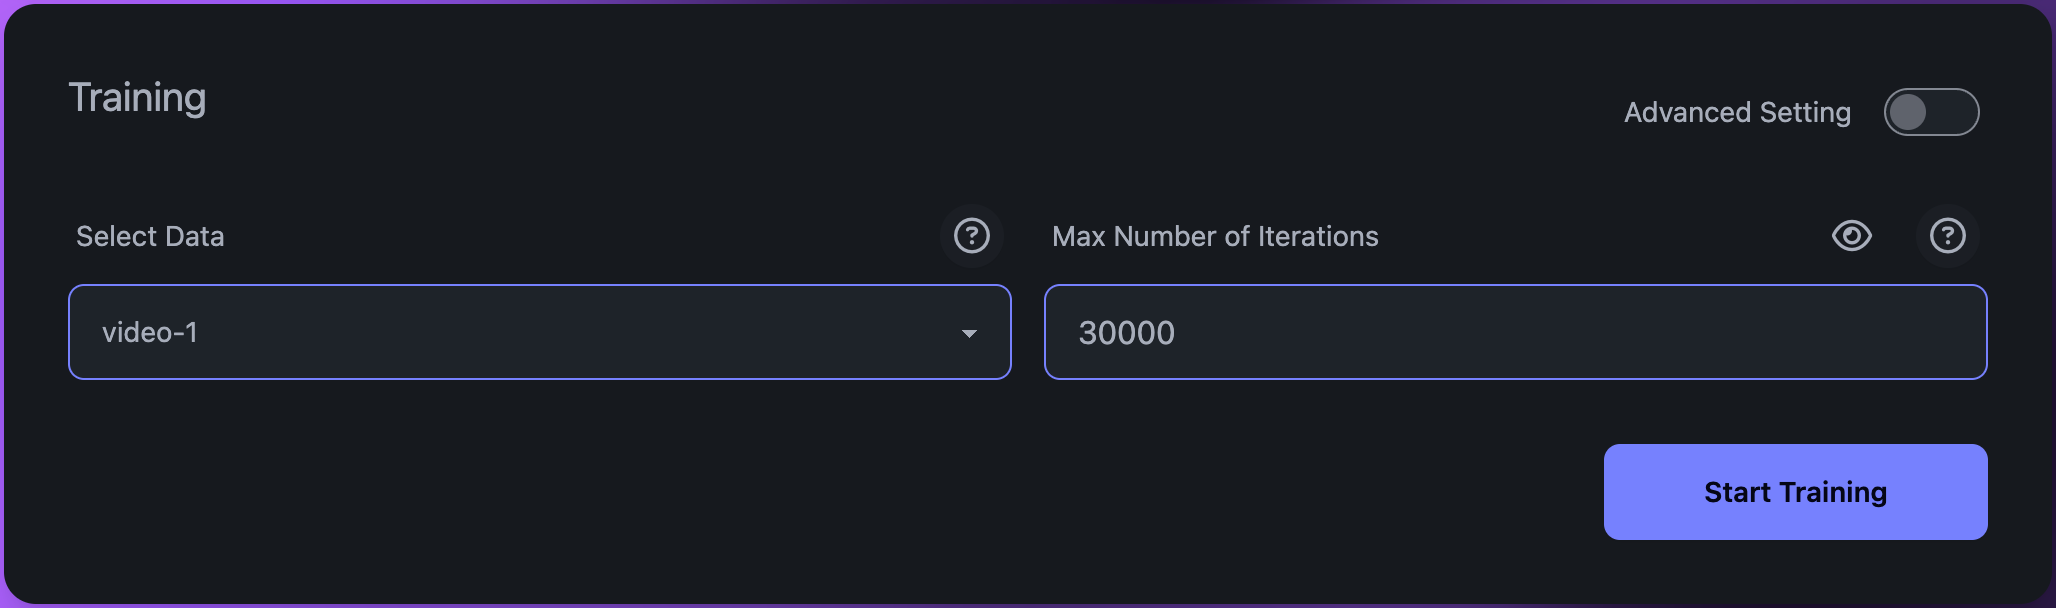
\includegraphics[width=.65\textwidth]{figures/fix-2.png}
% 	\caption{Consistent Wording for Training Button}
%   \label{fig:fix-2}
% \end{figure}

\cleanparagraph{Enhanced Project Creation}
The project creation process was moved into a modal dialog, which not only eliminates a point of confusion but also clarified the need to name projects before creation \fref{fig:fix-3}.

\begin{figure}[htb]
  \centering
	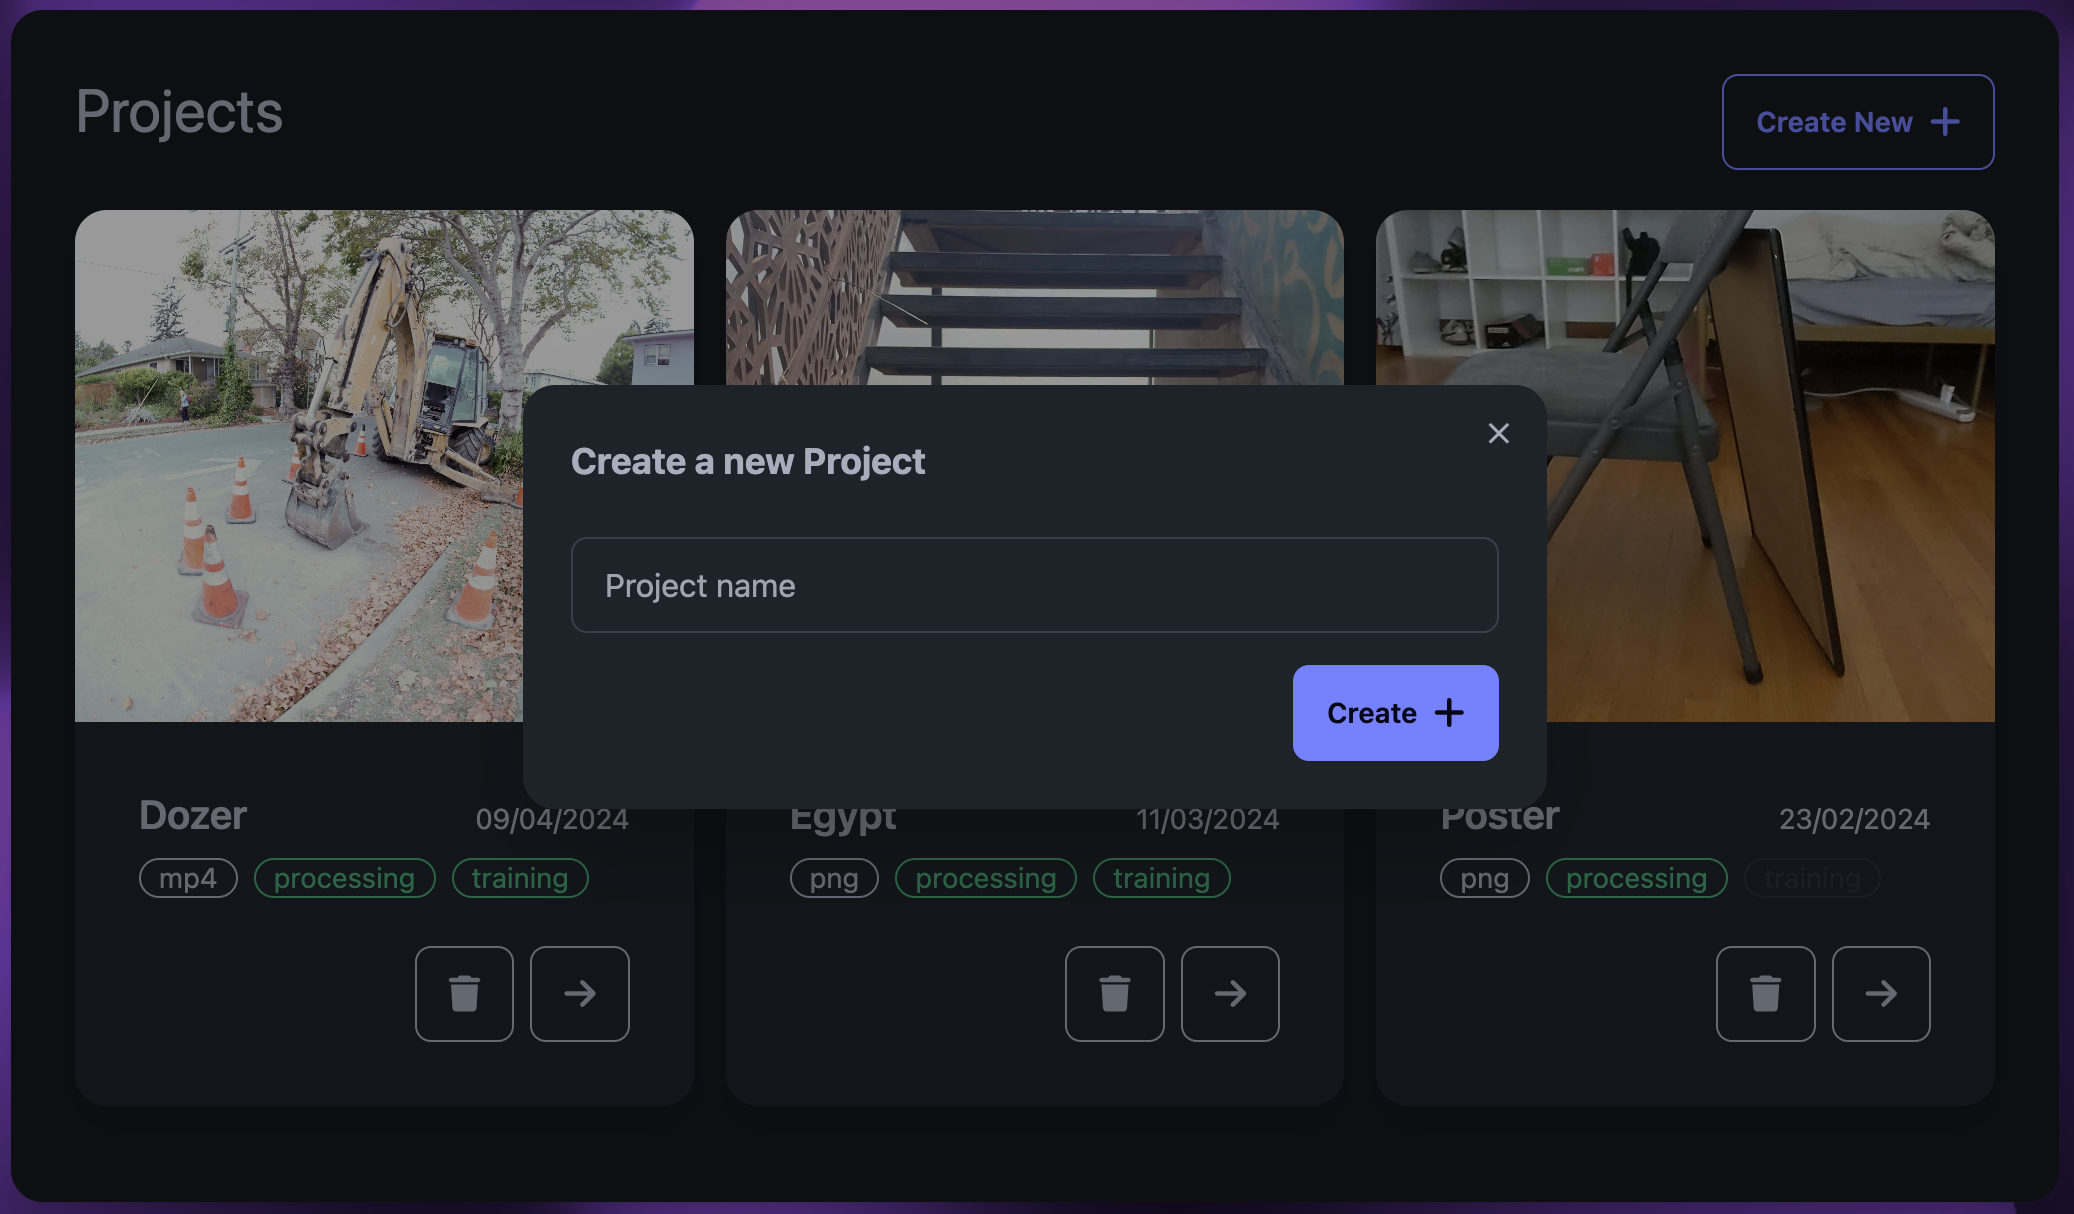
\includegraphics[width=.8\textwidth]{figures/fix-3.png}
	\caption{Modal Dialog for Project Creation.}
  \label{fig:fix-3}
\end{figure}

\cleanparagraph{File Upload Improvements}
The file upload process was improved by adding some guardrails, to ensure user would not accidentally skip a step.
The upload button starts out disabled, so that the only interactive element is the file-input field.
Once a file is selected, the button becomes active, indicating to the user that they can proceed to upload their selected file.
Only once the file is uploaded, the UI elements related to pre-processing appear, guiding the user through the next steps.
This solution is likely to prevent many of the issues users encountered when uploading files during testing \fref{fig:fix-4}.


\begin{figure}[htb]
  \begin{subfigure}{\textwidth}
    \centering
    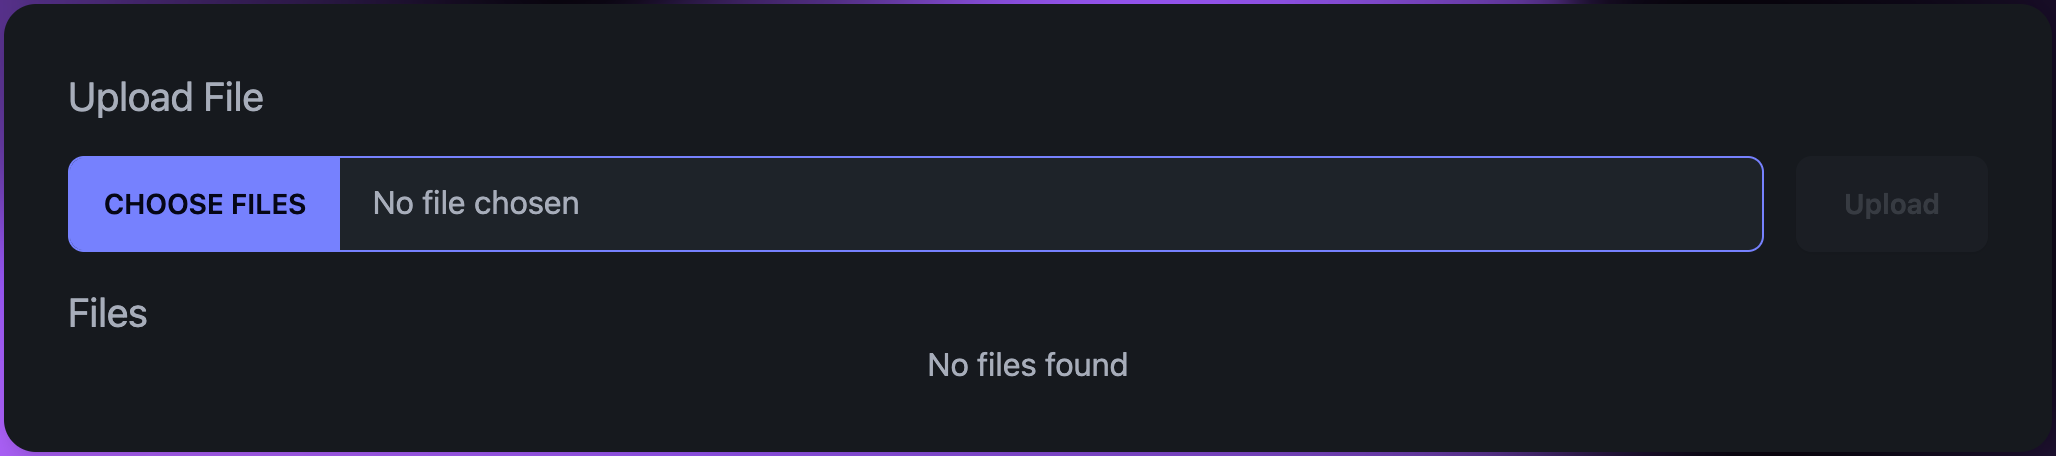
\includegraphics[width=.8\linewidth]{figures/fix-4.1.png}
    \caption{Initial State}
  \end{subfigure}
  \begin{subfigure}{\textwidth}
    \centering
    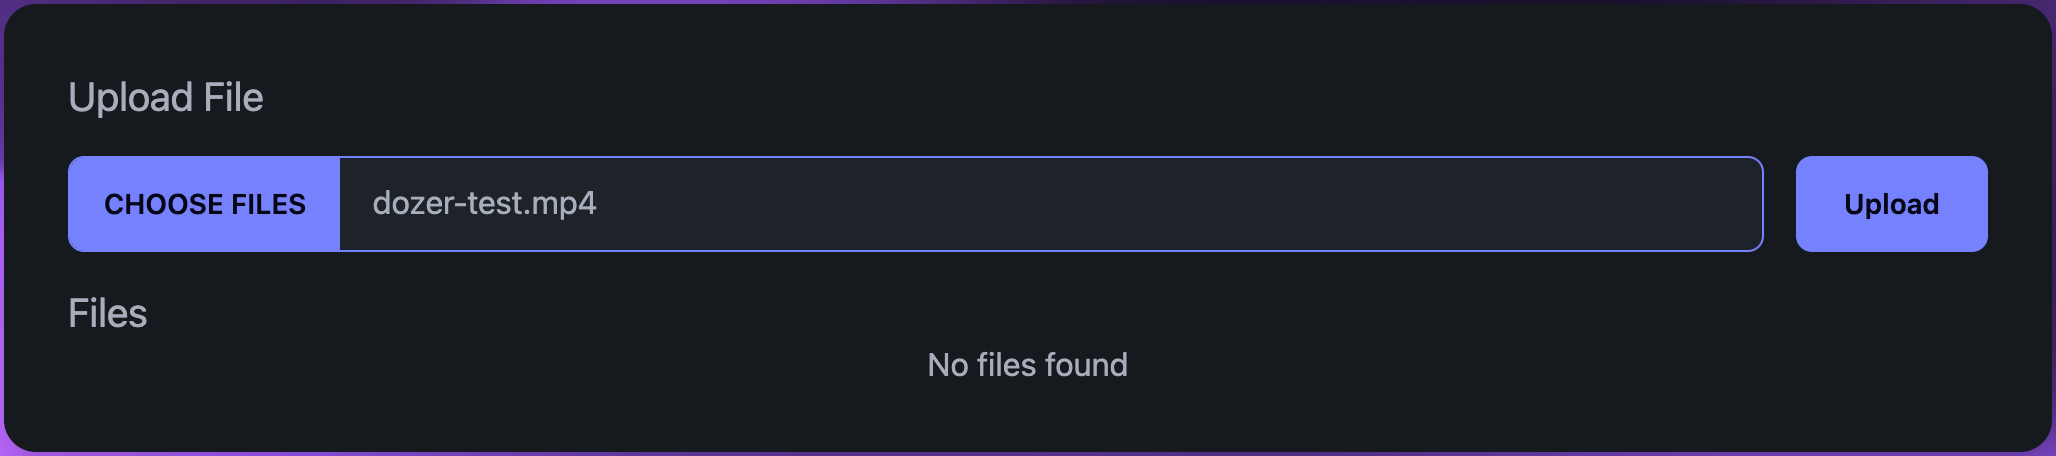
\includegraphics[width=.8\linewidth]{figures/fix-4.2.png}
    \caption{File Selected}
  \end{subfigure}
  \begin{subfigure}{\textwidth}
    \centering
    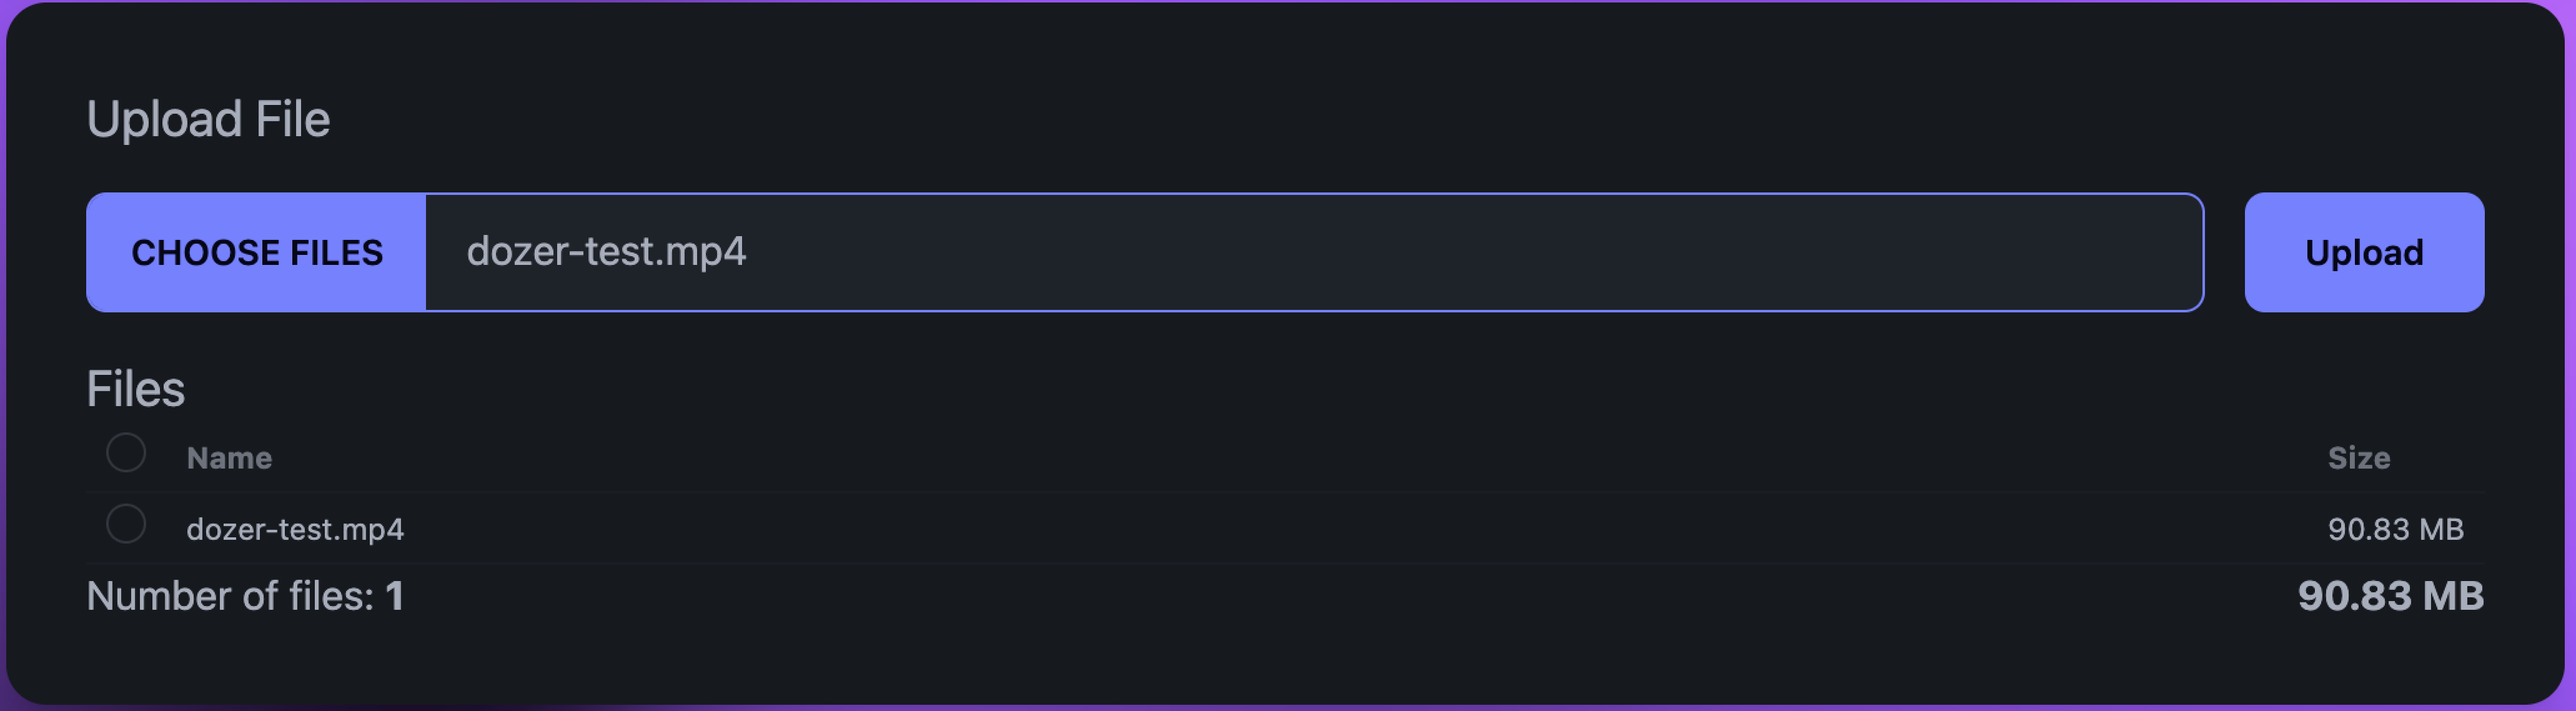
\includegraphics[width=.8\linewidth]{figures/fix-4.3.png}
    \caption{File Uploaded}
  \end{subfigure}
	\caption{Improved File Upload Process.}
  \label{fig:fix-4}
\end{figure}

\cleanparagraph{Disabling Background Animations}
A potential concern for some participants was the presence of background animations, which could be distracting to some users.
To address this, an option was added to disable background animations in a sub-menu accessible in the header \fref{fig:fix-5}.

\begin{figure}[htb]
  \centering
  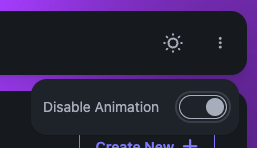
\includegraphics[width=.5\textwidth]{figures/fix-5.png}
  \caption{Option to Disable Background Animations.}
  \label{fig:fix-5}
\end{figure}